\documentclass[a4paper, 12pt]{article}

\usepackage{graphicx}
\usepackage{xcolor}
\usepackage{mdframed}
\usepackage { amsmath , amssymb , amsthm }
\usepackage[T2A]{fontenc}
\usepackage[utf8]{inputenc}
\usepackage[english,russian]{babel}

\graphicspath{{img/}}
\DeclareGraphicsExtensions{.pdf,.png,.jpg}


\title{экз}
\author{Осипенко}
\date{\today}

\begin{document}
\sffamily
\maketitle
\begin{center}
    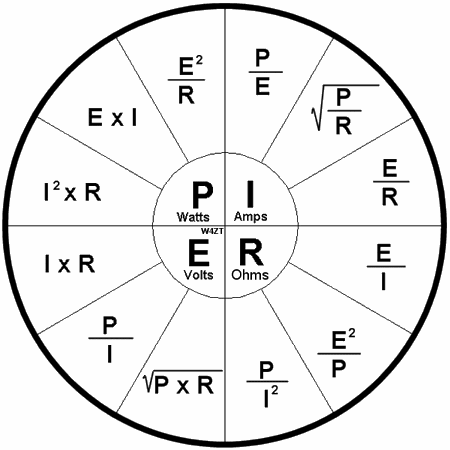
\includegraphics{int.png}
\end{center}
\section{Основные понятия и определения электрических цепей. Классификация цепей. Элементы цепи. Схема замещения, топология цепей.}
Электрической цепью называется совокупность электротехнических устройств, образующих путь для прохождения электрического тока. К электротехническим устройствам относятся:

    -источники электромагнитной энергии (генераторы) или источники электрических сигналов (гальванические элементы, аккумуляторы);

    -приемники или потребители;

    -устройства передачи и преобразования электрической энергии (кабели, провода и трансформаторы).

Поддерживать в проводниках постоянный электрический ток можно лишь в том случае, если создана замкнутая цепь из проводников и в этой цепи есть источник тока. Электротехнические устройства, производящие электрическую энергию, называются генераторами или источниками электрической энергии, а устройства, потребляющие ее – приемниками (потребителями) электрической энергии.\\

Классификациируют цепи \dots:\\
1)По роду тока: постоянного тока, переменного тока, синусоидальные, несинусоидальные.\\
2)По числу фаз: однофазные, трехфазные.\\
3)По характеру элементов: линейные (в них все элементы линейные), нелинейные (содержат хотя бы один нелинейный элемент)

Линейные элементы отличаются от нелинейных вольт-амперными характеристиками (ВАХ) $ I = f(U) $.

Основные топологические понятия:\\
-узел – место соединения трех и более ветвей;\\
-ветвь – участок цепи между двумя соседними узлами, в котором  все  элементы соединены последовательно;\\
-контур – замкнутый участок электрической цепи, в котором каждый из элементов цепи встречается не более одного раза.\\

Схема замещения - графическая модель электрической цепи с использованием и идеализированных элементов, необходима для расчета цепи.
\section{Пассивные и активные элементы схем замещения (определения, примеры).}
Активным называется элемент, содержащий в своей структуре источник электрической энергии. К пассивным относятся элементы, в которых рассеивается (резисторы) или накапливается (катушка индуктивности и конденсаторы) энергия. К основным характеристикам элементов цепи относятся их вольт-амперные, вебер-амперные и кулон-вольтные характеристики, описываемые дифференциальными или (и) алгебраическими уравнениями.\\
1)Резистор – это пассивный элемент, характеризующийся резистивным сопротивлением.\\
2)Катушка – это пассивный элемент, характеризующийся индуктивностью.\\
3)Конденсатор – это пассивный элемент, характеризующийся емкостью.
\section{Последовательное и параллельное соединение резисторов.}
Последовательное соединение резисторов это такое соединение, в котором конец одного резистора соединен с началом второго резистора, конец второго резистора с началом третьего и так далее. (Rобщ = R1 + R2 + R3+...+ Rn.)

Параллельное соединение резисторов это соединение, в котором начала всех резисторов соединены в одну общую точку (А), а концы в другую общую точку (Б). (1/Rобщ= 1/R1+1/R2+1/R3+…+1/Rn)

Смешанное соединение резисторов является комбинацией последовательного и параллельного соединения.
\section{Преобразование соединения резисторов треугольником в эквивалентную звезду и }
\section{преобразование соединения резисторов звездой в эквивалентный треугольник.}
Во многих схемах можно встретить такие конфигурации компонентов, в которых невозможно выделить последовательные или параллельные цепи. К этим конфигурациям относятся соединения компонентов в виде звезды и треугольника:\\
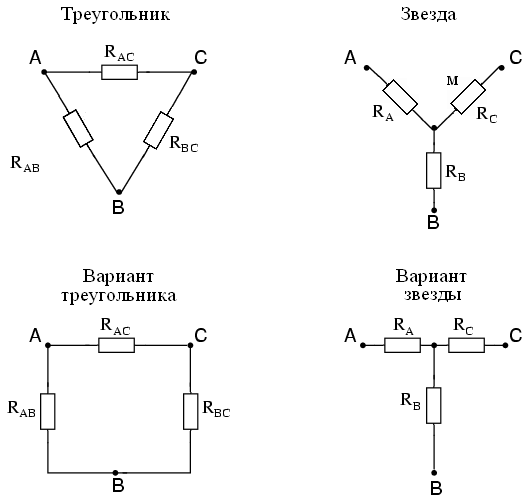
\includegraphics{4-1.png}\\
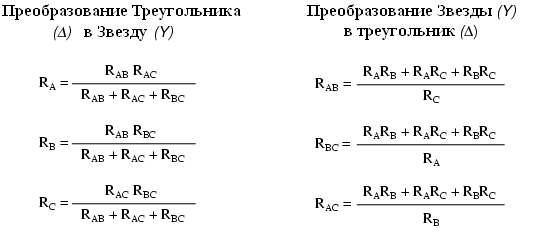
\includegraphics{4-2.png}\\
\section{Идеальный и реальный источник ЭДС. Свойства, нагрузочная характеристика.}
Идеальный источник, представляющий собой двухполюсник, на зажимах которого электродвижущая сила (и напряжение) всегда поддерживается постоянным значением. На него не влияет нагрузка сети, а внутреннее сопротивление у источника равно нулю. 

Теоретически на выводах у идеального источника напряжение не зависит от величины тока нагрузки и является постоянной величиной. Однако, это условная абстракция, которая не может быть осуществлена на практике. У реального источника при увеличении тока нагрузки значение напряжения на зажимах всегда уменьшается.\\ 
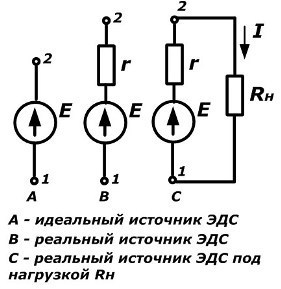
\includegraphics[scale=0.8]{6-1.png}\\
В действительности источниками напряжения работают различные химические и гальванические элементы, аккумуляторные батареи, электрические сети. Их разделяют на источники: 

    -постоянного и переменного напряжения; 

    -управляемые напряжением или током.
\section{Идеальный и реальный источник тока. Свойства, нагрузочная характеристика.}
Ими называют двухполюсники, создающий ток, который является строго постоянной величиной и никак не зависит от значения сопротивления на подключенной нагрузке, а внутреннее сопротивление его приближается к бесконечности. Это тоже теоретическое допущение, которое на практике не может быть достигнуто. 

Для идеального источника тока напряжение на его клеммах и мощность зависят только от сопротивления подключенной внешней схемы. При этом с увеличением сопротивления они возрастают. 

Реальный источник тока отличается от идеального значением внутреннего сопротивления.\\ 
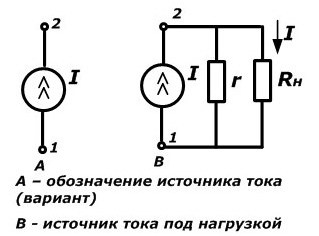
\includegraphics{7-1.png}
\section{Взаимные эквивалентные преобразования источников ЭДС и тока.}
При расчете электрических цепей иногда целесообразно произвести преобразование источника тока в источник напряжения и наоборот\\
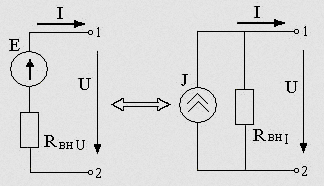
\includegraphics{8-1.png}\\
условие эквивалентности источников - $ J = E R_{BH} $\\
*реальному источнику Е, Rвh всегда можно найти реальный источник тока J, Rвh. Но идеальному источнику Е нельзя найти эквивалентный идеальный источник J, так как внутренние сопротивления у них не могут
быть одинаковыми.
\section{Последовательное и параллельное соединение источников ЭДС.}
\section{Параллельное и последовательное соединение источников тока.}
При последовательном соединении элементов питания выделяются две схемы: последовательно-дополняющая и последовательно-препятствующая.

В последовательно-дополняющей схеме положительный вывод первого элемента питания соединяется с отрицательным выводом второго элемента питания; положительный вывод второго элемента питания соединяется с отрицательным выводом третьего элемента питания и т.д.

При таком соединении источников питания через все элементы будет течь одинаковый ток:

\[
    I=I1=I2=I3    
\] 

Индексы в обозначениях токов указывают на номера отдельных источников питания (элементов или батарей питания)
А полное напряжение при последовательном соединении равно сумме напряжений (ЭДС) отдельных элементов:

\[
    E = E1 + E2 + E3.    
\] 

При последовательно-препятствующем включении источников питания, они соединяются друг с другом одноименными выводами. Но на практике такая схема не применяется или применяется, но очень редко.\\

При параллельном соединении элементов питания, их одноименные выводы соединяются вместе, то есть плюс к плюсу, минус к минусу.

В этом случае общий ток будет равен сумме токов каждого элемента:

\[
    I=I1+I2+I3
\]

Общее напряжение при параллельном включении источников питания будет равно напряжению каждого отдельного источника.

\[
       E = E1 + E2 + E3
\]

Источники питания включают по последовательно-параллельной схеме для увеличения, как тока, так и напряжения. При этом основываются на том, что параллельное включение увеличивает силу тока, а последовательное увеличивает общее напряжение.
\section{Пассивные и активные двухполюсники. Схемы замещения. Вольт-амперная (нагрузочная) характеристика линейного активного двухполюсника. Режимы работы активного двухполюсника (на характеристике).}
\section{Режим холостого хода и короткого замыкания активного двухполюсника. Определение параметров активного двухполюсника (Uхх, Iкз, Rэ)}
\section{Согласованный режим работы активного двухполюсника.}
Двухполюсником называется часть электрической цепи любой сложности и произвольной конфигурации, выделенная относительно двух зажимов (двух полюсов).

Двухполюсник, не содержащий источников энергии или содержащий скомпенсированные источники (суммарное действие которых равно нулю), называется пассивным. Если в схеме двухполюсника имеются нескомпенсированные источники, он называется активным. На схеме двухполюсник обозначают прямоугольником с двумя выводами. Это обозначение можно условно рассматривать как коробку, внутри которой находится электрическая цепь. 

Пассивный двухполюсник является потребителем энергии и может быть заменен эквивалентным сопротивлением, величина которого равна входному сопротивлению двухполюсника.\\

Зависимость напряжения на выводах пассивного двухполюсника от тока в нём (U=f(I)) называется нагрузочной характеристикой или вольт-амперной характеристикой (ВАХ). Так же как и внешняя характеристика активного двухполюсника вольт-амперная характеристика строится в координатах ток-напряжение и лежит в первом и третьем квадрантах.

ВАХ линейных двухполюсников представляет собой прямую линию, проходящую через начало координат. Уравнение линейной ВАХ: U=IR

В зависимости от нагрузки различают следующие режимы работы: номинальный, режим холостого хода, короткого замыкания, согласованный режим. Работа активного двухполюсника под нагрузкой Rн определяется его ВАХ, уравнение которой $ U = E - Ir_0 $ \\
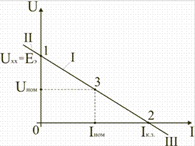
\includegraphics{11-1.png}

1-Режим холостого хода возникает при обрыве цепи или отключении сопротивления нагрузки.
\[
       U = U_{xx} = E
\]

2-Режим короткого замыкания получается при сопротивлении нагрузки, равном нулю. Ток короткого замыкания в несколько раз превышает номинальный ток. Режим короткого замыкания является аварийным.
\[
       I = \frac{E_0}{r} 
\]

-Номинальный режим электрической цепи обеспечивает технические параметры как отдельных элементов, так и всей цепи, указанные в технической документации, в справочной литературе или на самом элементе. Для разных электротехнических устройств указывают свои номинальные параметры. Однако три основных параметра указываются практически всегда: номинальное напряжение Uном, номинальная мощность Рном и номинальный ток Iном
\[
       Q = I^2 Rt
\]

-Согласованный режим - это режим передачи от источника к сопротивлению нагрузки наибольшей мощности. Согласованный режим наступает тогда, когда сопротивление нагрузки становится равным внутреннему сопротивлению источника. При этом в нагрузке выделяется максимальная мощность.

\section{КПД активного двухполюсника. КПД в согласованном режиме.}
КПД эквивалентного активного двухполюсника:\\
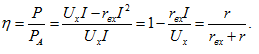
\includegraphics{14-1.png}\\
КПД в согласованном режиме:\\
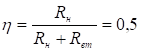
\includegraphics{14-2.png}
\section{Законы Ома (для участка цепи постоянного тока, замкнутой цепи, активной ветви).}

\section{1-й и 2-й законы Кирхгофа для цепей постоянного тока.}
1-Алгебраическая сумма всех токов в узле равна нулю.\\
2-Алгебраическая сумма ЭДС, действующих в замкнутом контуре, равна алгебраической сумме падений напряжения на всех резистивных элементах в этом контуре.\\
\section{Расчет цепей постоянного тока методом эквивалентных преобразований пассивных элементов и методом пропорциональных величин.}
Основными законами, определяющими расчет электрической цепи, являются законы Кирхгофа.

На основе законов Кирхгофа разработан ряд практических методов расчета электрических цепей постоянного тока, позволяющих сократить вычисления при расчете сложных схем.

Существенно упростить вычисления, а в некоторых случаях и снизить трудоемкость расчета, возможно с помощью эквивалентных преобразований схемы.

Преобразуют параллельные и последовательные соединения элементов, соединение «звезда» в эквивалентный «треугольник» и наоборот. Осуществляют замену источника тока эквивалентным источником ЭДС. Методом эквивалентных преобразований теоретически можно рассчитать любую цепь, и при этом использовать простые вычислительные средства. Или же определить ток в какой-либо одной ветви, без расчета токов других участков цепи.\\

Метод пропорциональных величин (метод пропорционального пересчета) применяют для нахождения неизвестных токов в линейных электрических цепях с одним источником ЭДС (или тока). Для этого задаются произвольной величиной тока в самой удаленной от источника ветви n (например током In*=1А), а затем последовательно перемещаясь от выбранной ветви к источнику находят все напряжения на разветвлениях и токи в ветвях. В результате получается некоторое условное значение напряжения (или тока) источника Uи*(или Jи*), которое вероятнее всего будет отличаться от заданного. Взяв отношение заданного значения источника Uи к полученному Uи*(или Jи к Jи*) определяют коэффициент пересчета (коэффициент подобия)\\
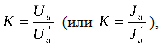
\includegraphics{15-1.png}\\
а действительные токи и напряжения на всех участках цепи находят умножив расчетные значения на коэффициент пересчета\\
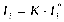
\includegraphics{15-2.png}\\
\section{Расчет цепей постоянного тока методом непосредственного использования законов Кирхгофа.}
Метод непосредственного применения правил Кирхгофа для расчета электрической цепи заключается в составлении системы из В уравнений с В неизвестными (B — количество ветвей в рассматриваемой цепи) по двум правилам Кирхгофа и последующем их решении.\\

Алгоритм:

    1)Определяем число узлов и ветвей в цепи и произвольным образом направляем токи в ветвях.

    2)Составляем максимально возможное число уравнений по первому закону Кирхгофа (на единицу меньше числа узлов).
    
    3)Недостающие уравнения составляем  по  второму закону Кирхгофа (общее число уравнений должно быть равно числу неизвестных токов, т.е. числу ветвей).

    4)Решая полученную  систему  линейных  уравнений, определяем неизвестные токи.

\section{Расчет цепей постоянного тока методом контурных токов.}
В методе контурных токов за неизвестные величины принимаются расчетные (контурные) токи, которые якобы протекают в каждом из независимых контуров. Таким образом, количество неизвестных токов и уравнений в системе равно числу независимых контуров цепи.

Расчет токов ветвей по методу контурных токов выполняют в следующем порядке:

1 Вычерчиваем принципиальную схему цепи и обозначаем все элементы.

2 Определяем все независимые контуры.

3 Произвольно задаемся направлением протекания контурных токов в каждом из независимых контуров (по часовой стрелке или против). Обозначаем эти токи. Для нумерации контурных токов можно использовать арабские сдвоенные цифры (I11, I22, I33 и т. д.) или римские цифры.

4 По второму закону Кирхгофа, относительно контурных токов, составляем уравнения для всех независимых контуров. При записи равенства считать, что направление обхода контура, для которого составляется уравнение, совпадает с направлением контурного тока данного контура. Следует учитывать и тот факт, что в смежных ветвях, принадлежащих двум контурам, протекают два контурных тока. Падение напряжения на потребителях в таких ветвях надо брать от каждого тока в отдельности.

5 Решаем любым методом полученную систему относительно контурных токов и определяем их.

6 Произвольно задаемся направлением реальных токов всех ветвей и обозначаем их. Маркировать реальные токи надо таким образом, чтобы не путать с контурными. Для нумерации реальных токов можно использовать одиночные арабские цифры (I1, I2, I3 и т. д.).

7 Переходим от контурных токов к реальным, считая, что реальный ток ветви равен алгебраической сумме контурных токов, протекающих по данной ветви.

При алгебраическом суммировании без изменения знака берется контурный ток, направление которого совпадает с принятым направлением реального тока ветви. В противном случае контурный ток умножается на минус единицу. 

\section{Расчет цепей постоянного тока методом узловых потенциалов.}
Метод узловых потенциалов – один из методов анализа электрической цепи, который целесообразно использовать, когда количество узлов в цепи меньше или равно числу независимых контуров. Данный метод основан на составлении уравнений по первому закону Кирхгофа. При этом, потенциал одного из узлов цепи принимается равным нулю, что позволяет сократить число уравнений до n-1.
\section{Расчет цепей постоянного тока методом двух узлов.}
Метод двух узлов - метод расчета электрических цепей, в котором за искомое (с его помощью определяют затем и токи ветвей) принимают напряжение между двумя узлами схемы.

Часто встречаются схемы, содержащие всего два узла. Наиболее рациональным методом расчета токов в них является метод двух узлов.

Формула для расчета напряжения между двумя узлами:

    \[
        U a b = {{\Sigma E_{k}g_{k}} \over {\Sigma g_{k}}}
    \]

где Ek - напряжение источника ЭДС k-той ветви, а gk - проводимость k-той ветви. 
\section{Расчет цепей постоянного тока методом наложения.}
Метод наложения - метод расчёта электрических цепей, основанный на предположении, что электрический ток в каждой из ветвей электрической цепи при всех включённых генераторах равен сумме токов в этой же ветви, полученных при включении каждого из генераторов по очереди и отключении остальных генераторов (только в линейных цепях).

Метод наложения используется как для расчёта цепей постоянного тока, так и для расчёта цепей переменного тока. 
\section{Расчет цепей постоянного тока методом эквивалентного генератора.}
Метод эквивалентного генератора используется при расчёте сложных схем, в которых одна ветвь выделяется в качестве сопротивления нагрузки, и требуется исследовать и получить зависимость токов в цепи от величины сопротивления нагрузки.

В соответствии с данным методом неизменная часть схемы преобразовывается к одной ветви, содержащей ЭДС и внутреннее сопротивление эквивалентного генератора.

Применение метода эквивалентного генератора

ЭДС эквивалентного генератора определяется по формуле:

\[
    E e q v ={\frac {{E_{1}G_{1}}+{E_{2}G_{2}}+{E_{3}G_{3}}+\ldots +{E_{n}G_{n}}}{G_{1}+G_{2}+G_{3}+\ldots +G_{n}}}
\]

где: $ G_{i} $ - проводимость участка цепи, равная 1 R i $ \frac{1}{R_i} $.

Для определения эквивалентного сопротивления генератора применяется расчет последовательно и параллельно соединённых сопротивлений, а также, в случае более сложных схем, применяют преобразование треугольник-звезда.

После определения параметров эквивалентного генератора можно определить ток в нагрузке при любом значении сопротивления нагрузки по формуле:

\[
    I_H = \frac{E_{eqv}}{R_{eqv}} + R_H
\]

Любой сколь угодно сложный активный двухполюсник можно представить эквивалентным генератором, ЭДС которого равна напряжению холостого хода на зажимах двухполюсника, а внутреннее сопротивление равно входному сопротивлению пассивного двухполюсника со стороны тех же зажимов. При определении входного сопротивления все источники должны быть заменены своими внутренними сопротивлениями - источники ЭДС закорачиваются, а источники тока размыкаются.
\section{Расчет цепей постоянного тока методом эквивалентных преобразований источников энергии.}
 
\section{Принципы компенсации напряжения и тока. Потенциальная диаграмма цепи постоянного тока.}
Принцип компенсации основан на теореме о компенсации, которая гласит: в любой электрической цепи без изменения токов в ее ветвях сопротивление в произвольной ветви можно заменить источником с ЭДС, численно равной падению напряжения на этом сопротивлении и действующей навстречу току в этой ветви.\\

Потенциальной диаграммой называется графическое изображение распределения электрического потенциала вдоль замкнутого контура в зависимости от сопротивления участков, входящих в выбранный контур. 

Для построения потенциальной диаграммы выбирают замкнутый контур. Этот контур разбивают на участки таким образом, чтобы на участке находился один потребитель или источник энергии. Пограничные точки между участками необходимо обозначить буквами или цифрами.

Произвольно заземляют одну точку контура, её потенциал условно считается нулевым. Обходя контур по часовой стрелке от точки с нулевым потенциалом, определяют потенциал каждой последующей пограничной точки как алгебраической суммы потенциала предыдущей точки и изменения потенциала между этими соседними точками.

мультиметрИзменение потенциала на участке зависит от состава цепи между точками. Если на участке включен потребитель энергии (резистор), то изменение потенциала численно равно падению напряжения на этом резисторе. Знак этого изменения определяют направлением тока. При совпадении направлений тока и обхода контура знак отрицательный, в противном случае он положительный.

Если на участке находится источник ЭДС, то изменение потенциала здесь численно равно величине ЭДС данного источника. При совпадении направления обхода контура и направления ЭДС изменение потенциала положительно, в противном случае оно отрицательно.

После расчета потенциалов всех точек строят в прямоугольной системе координат потенциальную диаграмму. На оси абсцисс откладывают в масштабе сопротивление участков в той последовательности, в которой они встречались при обходе контура, а по оси ординат – потенциалы соответствующих точек. Потенциальная диаграмма начинается с нулевого потенциала и заканчивается после обхода контура таковым. \\
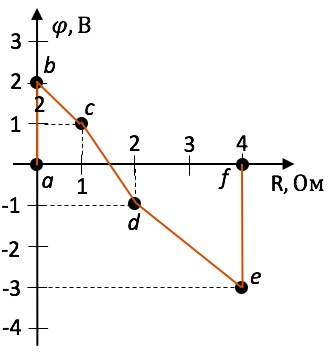
\includegraphics{25-1.png}
\section{Баланс мощностей в цепи постоянного тока.}
Баланс мощностей – это выражение закона сохранения энергии, в электрической цепи. Определение баланса мощностей звучит так: сумма мощностей потребляемых приемниками, равна сумме мощностей отдаваемых источниками. То есть если источник ЭДС в цепи отдает 100 Вт, то приемники в этой цепи потребляют ровно такую же мощность. 

Баланс мощностей используют для проверки правильности расчета электрических цепей. 
\section{Преимущества цепей переменного тока. Способы представления синусоидальных токов, напряжений, ЭДС.}
Переменный ток легче получить и передать на дальние расстояния. Также он хорошо трансформируется, то есть достаточно просто повысить или понизить его напряжение. \\

В современной технике широко используют разнообразные по форме переменные токи и напряжения: синусоидальные, прямоугольные, треугольные и др. Значение тока, напряжения, ЭДС в любой момент времени t называется мгновенным значением и обозначается малыми строчными буквами, соответственно

i = i(t); u = u(t); e = e(t).

Токи, напряжения и ЭДС, мгновенные значения которых повторяются через равные промежутки времени, называют периодическими, а наименьший промежуток времени, через который эти повторения происходят, называют периодом Т.

Если кривая изменения периодического тока описывается синусоидой, то ток называют синусоидальным. Если кривая отличается от синусоиды, то ток несинусоидальный.


В промышленных масштабах электрическая энергия производится, передается и расходуется потребителями в виде синусоидальных токов, напряжений и ЭДС,

При расчете и анализе электрических цепей применяют несколько способов представления синусоидальных электрических величин.

\subsection{ Аналитический способ}
\begin{equation*}
    i(t) = I_m \sin(\omega t + \phi_i),
    u(t) = U_m \sin(\omega t + \phi_i),
    e(t) = E_m \sin(\omega t + \phi_i),
\end{equation*}
\subsection{Временная диаграмма}
Временная диаграмма представляет графическое изображение синусоидальной величины в заданном масштабе в зависимости от времени
\subsection{Графоаналитический способ}
Графически синусоидальные величины изображаются в виде вращающегося вектора. Предполагается вращение против часовой стрелки с частотой вращения $ \omega $. Величина вектора в заданном масштабе представляет амплитудное значение. Проекция на вертикальную ось есть мгновенное значение величины.

Совокупность векторов, изображающих синусоидальные величины (ток, напряжение, ЭДС) одной и той же частоты называют векторной диаграммой.

Векторные величины отмечаются точкой над соответствующими переменными.

Использование векторных диаграмм позволяет существенно упросить анализ цепей переменного тока, сделать его простым и наглядным.

В основе графоаналитического способа анализа цепей переменного тока лежит построение векторных диаграмм.
\subsection{Аналитический метод с использованием комплексных чисел}
Синусоидальный ток $ i(t) = I_m \sin(\omega t + \phi_i) $ можно представить комплексным числом $ I_m' $ на комплексной плоскости

\[
    I_m' = i_m e^{j\phi}
\]

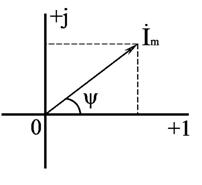
\includegraphics{27-1.png}\\

где амплитуда тока Im – модуль, а угол $ \phi $, являющийся начальной фазой, – аргумент комплексного тока.

Использование комплексной формы представления позволяет заменить геометрические операции над векторами алгебраическими операциями над комплексными числами. В результате этого к анализу цепей переменного тока могут быть применены все методы анализа цепей постоянного тока.
\section{Действующее и среднее значения переменного тока.}
Под действующим значением переменного тока  понимают  значение постоянного тока I, который, проходя по резистору, выделяет в нем такое же количество тепла, что и действительный синусоидальный ток $ i(t) = I_m \sin(\omega t + \phi_i) $\\

Действующее:
\begin{equation*}
    I = I_m /\sqrt{2},
    U = U_m /\sqrt{2},
    E = E_m /\sqrt{2},
\end{equation*}

Среднее:
\begin{equation*}
    I_{\text{avg}} = I_m 2 / \pi,
    U_{\text{avg}} = U_m 2 / \pi,
    E_{\text{avg}} = E_m 2 / \pi,
\end{equation*}

\section{Идеальная и реальная индуктивность в цепи переменного тока.}
так как переменный ток непрерывно изменяется, то непрерывно возникающая в катушке ЭДС самоиндукции создает сопротивление переменному току. 

скорость изменения тока уменьшается по мере увеличения тока и увеличивается по мере его уменьшения, независимо от направления тока в цепи. 

ЭДС самоиндукции, вызываемая самим переменным током, препятствует его возрастанию и, наоборот, поддерживает его при убывании. 

в катушке индуктивности, включенной в цепь переменного тока, создается сопротивление прохождению тока. Но так как такое сопротивление вызывается в конечном счете индуктивностью катушки, то и называется оно индуктивным сопротивлением. 
\section{Идеальная и реальная емкость в цепи переменного тока.}
В цепи постоянного тока емкость (идеальный конденсатор) имеет сопротивление бесконечно большое, так как после окончания процесса заряда такой конденсатор не пропускает электрический ток. Однако при подключении емкости к источнику переменного тока происходит непрерывный процесс его заряда и разряда, при этом через емкость проходит переменный ток.
\section{Закон Ома, 1-й и 2-й законы Кирхгофа в комплексной форме. Векторные диаграммы.}
Первый закон Кирхгофа: «алгебраическая сумма комплексов тока в узле электрической цепи равна нулю» \\
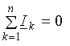
\includegraphics{30-1.png}\\
Второй закон Кирхгофа: «в любом замкнутом контуре электрической цепи алгебраическая сумма комплексных ЭДС равна алгебраической сумме комплексных напряжений на всех пассивных элементах этого контура». \\
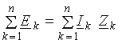
\includegraphics{30-2.png}\\

Закон Ома\\
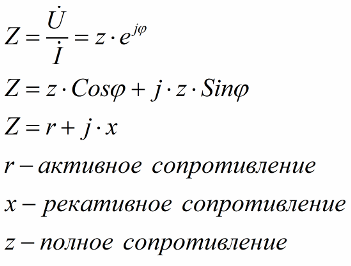
\includegraphics{30-3.png}\\

Векторная диаграмма - графическое изображение меняющихся по закону синуса (косинуса) величин и соотношений между ними при помощи направленных отрезков - векторов.
\section{Последовательное соединение R, L, C - элементов. Треугольники сопротивлений и напряжений.}
\section{}
\section{}
\section{}
\section{}
\section{}
\section{}
\section{}
\section{}
\section{}
\section{}
\section{}
\section{}
\section{}
\section{}
\section{}
\section{}
\section{}
\section{}
\section{}
\section{}
\section{}
\section{}
\section{}
\section{}
\section{}
\section{}
\section{}
\section{}
\section{}
\section{}
\section{}



\end{document}